\documentclass{article}
\usepackage[UTF8]{ctex}
\usepackage{geometry}
\usepackage{makecell}
\usepackage{amsmath}
\usepackage{graphicx}
\usepackage{bigstrut}
\usepackage{subfigure}
\usepackage{float}
\usepackage{booktabs}
\usepackage{hyperref}
\usepackage{xcolor}
\definecolor{linkcolour}{rgb}{0,0.2,0.6}
\hypersetup{colorlinks,breaklinks,urlcolor=linkcolour, linkcolor=linkcolour}

\geometry{a4paper,scale=0.75}

\title{\heiti 实验三十\ 用示波器观测动态磁滞回线}
\author{\kaishu 田睿轩\ 物理学院\ 1900011602}
\date{2021年6月2日}
\newcommand{\degree}{^\circ}
\newcommand{\degreesCelsius}{^\circ C}

\begin{document}
    \maketitle
    \section{数据处理}
    \subsection{100Hz下铁氧体饱和磁滞回线}
    电路中各参数如下所示:
    $$R_1=2\Omega,R_2=50k\Omega,N=150,C=10\mu F,l=0.13m,S=1.24\times 10^{-4}m^2$$

    测量$f=100Hz$时的磁滞回线,调节励磁电流的电源电压幅度,使得磁化达到饱和,在示波器屏幕上显示出李萨如曲线,
    在上下半支上各测量9个以上的点的$u_{R_1}$和$u_c$然后利用如下公式计算出磁场强度和磁感应强度:
    $$H=\frac{N_{1}}{l R_{1}} u_{R_{1}}\ ,\ B=\frac{R_{2} C}{N_{2} S} u_{C}$$
    然后绘制出饱和磁滞回线。实验数据如表1所示,根据数据绘制的饱和磁滞回线如图1所示

    \begin{figure*}[h]
        \centering
        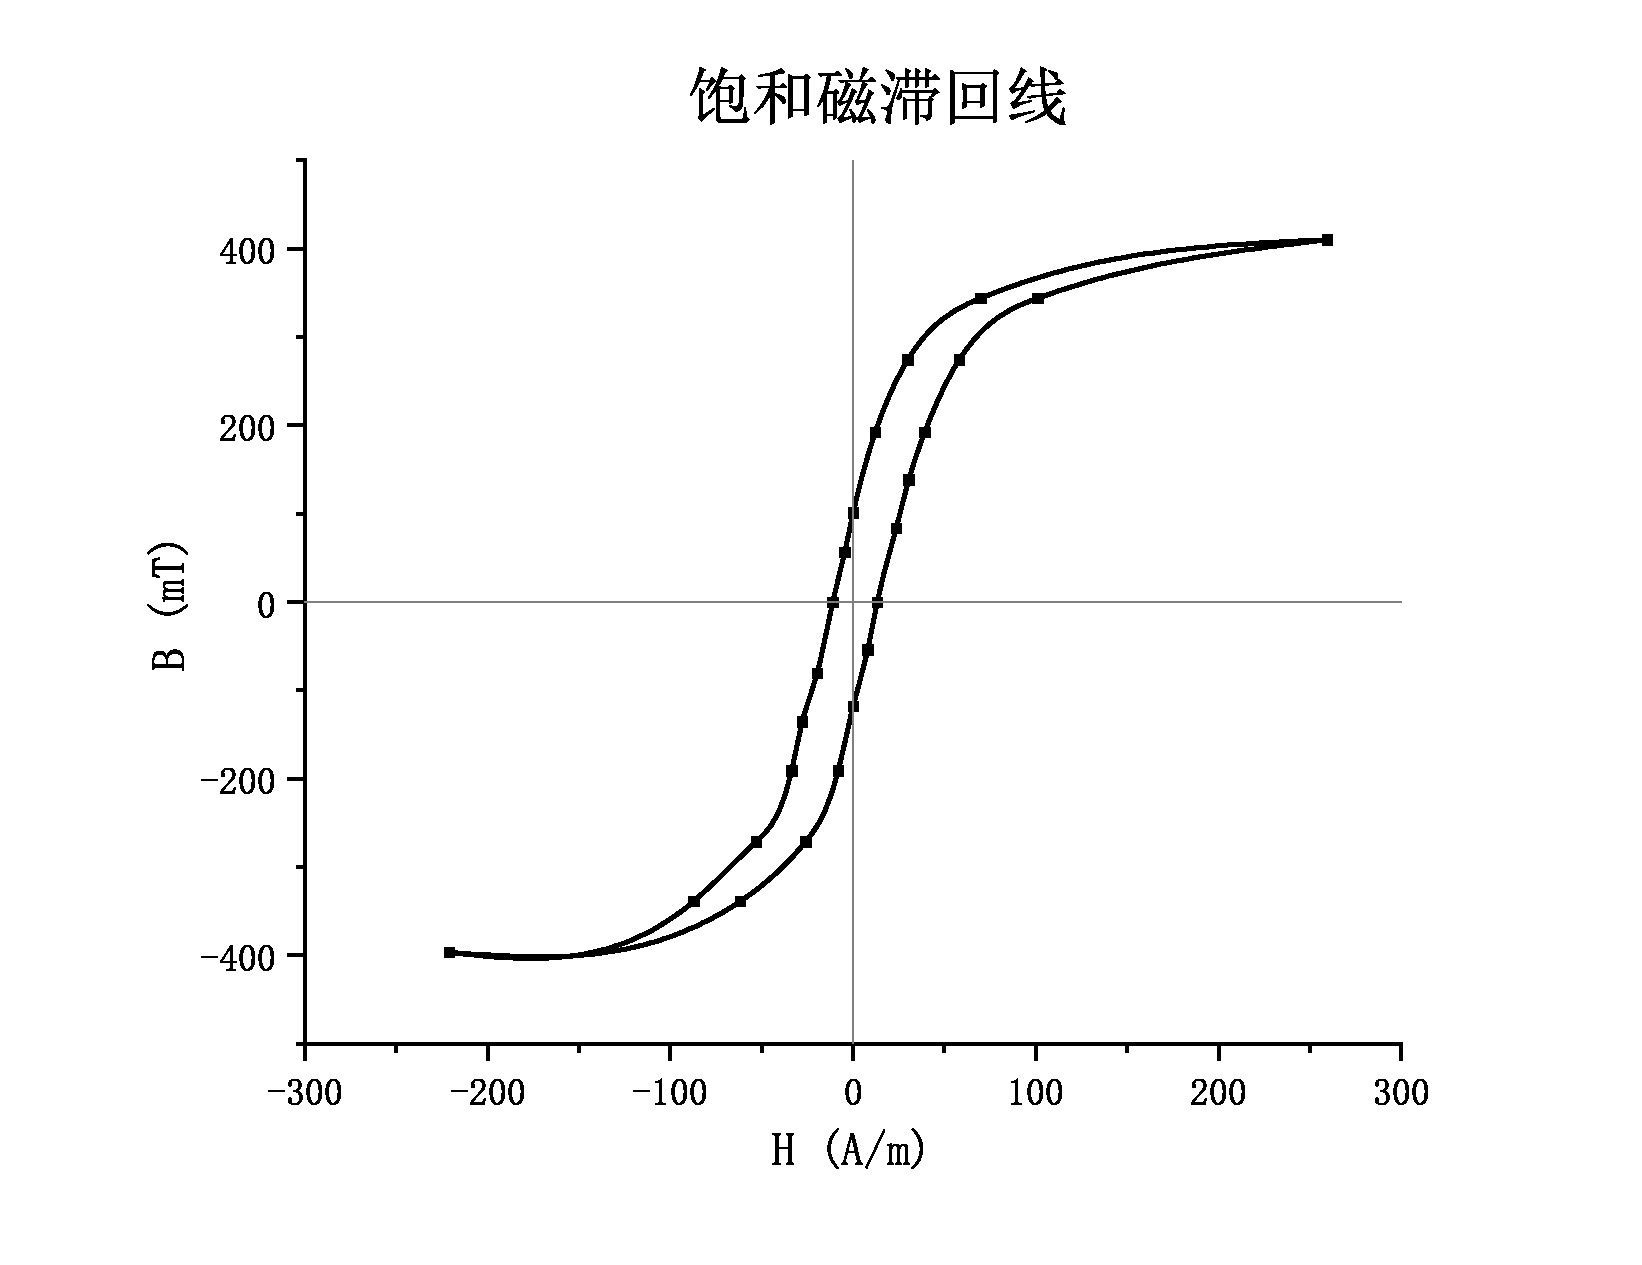
\includegraphics[width=0.6\textwidth]{饱和磁滞回线.eps}
        \caption{100Hz下饱和磁滞回线}
    \end{figure*}

    \newpage
    \begin{table}[h]
        \centering
        \caption{100Hz下饱和磁滞回线测量数据}
        \vspace{1ex}
        \begin{tabular}{ccccc}
            \toprule
            测量次数  & $u_{R_1}/(mV)$ & $H(A/m)$ & $u_c(mV)$ & $B(mT)$ \\
            \midrule
            1     & 450  & 260  & 15.25  & 410  \\
            2     & 121  & 70.0  & 12.80  & 344  \\
            3     & 52.0  & 30.0  & 10.20  & 274  \\
            4     & 21.0  & 12.1  & 7.15  & 192  \\
            5     & 0.0   & 0.00  & 3.75  & 101  \\
            6     & -8.0  & -4.62  & 2.10  & 56.5  \\
            7     & -19.0  & -11.0  & 0.00  & 0.00  \\
            8     & -34.0  & -19.6  & -3.00  & -80.6  \\
            9     & -48.0  & -27.7  & -5.05  & -136  \\
            10    & -58.0  & -33.5  & -7.10  & -191  \\
            11    & -92.0  & -53.1  & -10.10  & -272  \\
            12    & -151  & -87.1  & -12.60  & -339  \\
            13    & -383  & -221  & -14.75  & -396  \\
            14    & -107  & -61.7  & -12.60  & -339  \\
            15    & -45.0  & -26.0  & -10.10  & -272  \\
            16    & -14.0  & -8.08  & -7.10  & -191  \\
            17    & 0.0   & 0.00  & -4.40  & -118  \\
            18    & 14.0  & 8.08  & -2.00  & -53.8  \\
            19    & 23.0  & 13.3  & 0.00  & 0.00  \\
            20    & 41.0  & 23.7  & 3.10  & 83.3  \\
            21    & 53.0  & 30.6  & 5.15  & 138  \\
            22    & 68.0  & 39.2  & 7.15  & 192  \\
            23    & 101  & 58.3  & 10.20  & 274  \\
            24    & 175  & 101  & 12.80  & 344  \\
            \bottomrule
        \end{tabular}%    
    \end{table}

    表格中记录了饱和磁感应强度、剩磁和矫顽力的测量数据,摘录如下:
    
    \begin{enumerate}
        \item [(1)] 饱和磁感应强度:\\
        $$2u_{C}=30mV,B_{S}=403mT$$

        \item [(2)] 剩磁:\\
        $$u_{C}=8.15mV,B_{r}=114mT$$

        \item [(3)] 矫顽力:\\
        $$u_{R1}=42mV,H_{C}=12.2$$
    \end{enumerate}

    \subsection{不同频率下的饱和磁化曲线}
    分别测量$f=50,100,150Hz$时的饱和磁化曲线,测量出不同频率下的剩磁和矫顽力。

    $f=50Hz$时的$B_r$和$H_C$如下:
    $$2u_{C}=8.30mV,B_{r}=112mT$$
    $$2u_{R1}=44.0mV,H_{C}=12.7A/m$$

    $f=100Hz$时的$B_r$和$H_C$如下:
    $$2u_{C}=8.15mV,B_{r}=114mT$$
    $$2u_{R1}=42.0mV,H_{C}=12.2A/m$$

    $f=150Hz$时的$B_r$和$H_C$如下:
    $$2u_{C}=8.20mV,B_{r}=116mT$$
    $$2u_{R1}=44.0mV,H_{C}=12.7A/m$$

    在测量上述数据时,示波器横轴方向测量的满刻度值为1000mV,纵轴方向为40mV。而横轴方向测量的线宽约为10mV,纵轴方向约为0.5mV。
    示波器的仪器误差为测量值的2\%加满刻度值的0.3\%,将这两者的误差再复合上线宽带来的误差即可得电压测量的误差。
    
    测量剩磁的不确定度约为
    $$e_{2u_c}\approx2\%\times 8.2+0.3\% \times 40+0.5\approx 0.8mV$$
    $$\frac{\sigma_{2u_c}}{2u_c}=\frac{0.8/\sqrt{3}}{8.2}\approx6\%$$
    $$\frac{\sigma_{B_r}}{B_r}=\frac{\sigma_{2u_c}}{2u_c}\approx 6\%,\sigma_{B_r}\approx 7mT$$

    测量矫顽力时的不确定度约为
    $$e_{2u_{R_1}}\approx2\%\times 44.0+0.3\% \times 1000+10\approx 14mV$$
    $$\frac{\sigma_{2u_{R_1}}}{2u_{R_1}}=\frac{14/\sqrt{3}}{44}\approx18\%$$
    $$\frac{\sigma_{H_C}}{H_C}=\frac{\sigma_{2u_{R_1}}}{2u_{R_1}}\approx 18\%,\sigma_{B_r}\approx 2.3A/m$$

    从实验测得的数据可以看出,随着频率的增大,剩磁$B_r$略微增大,而矫顽力$H_C$几乎没有变化。这是因为材料的涡流损耗会随着频率的提升而增加,反映在磁滞回线上即为剩磁增大引起的磁滞回线围成的面积增加。
    但实验所用的样品1为铁氧体,涡流损耗很小,因此剩磁增大的不明显。

    \subsection{积分常量对曲线的影响}
    在$f=50Hz$下,固定励磁电流幅度为$I_m=0.2A$,即固定$u_m=0.4V$,改变积分常量,观察积分常量对李萨如图形的影响。积分常量为0.5s,0.05s,0.01s时的李萨如图形分别如图2、3、4所示。

    可以看到,随着时间常数$\tau=R_2C$的减小,李萨如图形在纵向被拉伸(三张图片中图形纵向占的格子数大致相等,但每格的电压值逐渐增大,因此如果放在相同比例下,图形会显示出逐渐拉伸的变化特点)。
    这是因为$B=\frac{R_{2} C}{N_{2} S} u_{C}$在B不变的情况下,$\tau$减小则$u_c$需要相应增大。

    此外,可以看到随着时间常数的减小,图形出现明显畸变,靠近原点处两条线逐渐重合,靠近饱和磁化处两条线距离增大。这是因为随着时间常数的减小,已经不满足$\tau\gg T=\frac{1}{f}$,
    电容上充放电不完全,$B=\frac{R_{2} C}{N_{2} S} u_{C}$的关系不再成立。

    不过这并不会改变真实的磁滞回线的形状。因为真实的磁滞回线的形状只受材料和磁化电流的频率、幅值的影响,这几个参数并没有变化。改变时间常数改变的是B到$u_C$之间的映射关系,因此李萨如图形会不一样。

    \begin{figure*}[htb]
        \centering
        \begin{minipage}{0.48\textwidth}
            \includegraphics[width=\textwidth]{0.5s.jpg}
            \caption{$\tau=50k\Omega\times 10\mu F=0.5s$} 
        \end{minipage}
        \begin{minipage}{0.48\textwidth}
            \includegraphics[width=\textwidth]{0.05s.jpg}
            \caption{$\tau=5k\Omega\times 10\mu F=0.05s$} 
        \end{minipage}
    \end{figure*}
    
    \begin{figure*}[htb]
        \centering
        \includegraphics[width=0.48\textwidth]{0.01s.jpg}
        \caption{$\tau=5k\Omega\times 2\mu F=0.01s$}
    \end{figure*}

    \subsection{动态磁化曲线}
    测量100Hz下的动态磁化曲线。控制励磁电流的幅值从小到大变化,测量20组$H_m$和$B_m$从而得到动态磁化曲线。实验数据如表2所示。
    
    根据测得数据绘制动态磁化曲线($B_m-H_m$曲线)和$\mu_m-H_m$曲线。分别图图5和图6所示。

    观察两张图可以发现,$B_m$随着$H_m$增大而增大,一开始增长比较慢,然后增加比较快,之后增长又减缓。
    $\mu_m-H_m$实质上是$B_m-H_m$曲线割线斜率随$H_m$的变化,因此$\mu_m-H_m$曲线上$\mu_m$随$H_m$先增大后减小。
    
    实验中测得,初始磁导率$\mu_i=3318$,最大磁导率为$\mu_{max}=4434$。

    \begin{table}[htb]
        \centering
        \caption{动态磁化曲线测量数据}
        \vspace{1ex}
        \begin{tabular}{cccccc}
            \toprule
            测量次数  & $2u_{R_1}/(mV)$ & $H_m(A/m)$ & $2u_c(mV)$ & $B_m(mT)$ & $\mu=\frac{B_m}{\mu_0H_m}$ \\
            \midrule
            1     & 9.40  & 2.71  & 0.84  & 11.3  & 3313  \\
            2     & 17.6  & 5.08  & 1.62  & 21.8  & 3413  \\
            3     & 23.2  & 6.69  & 2.26  & 30.4  & 3612  \\
            4     & 28.8  & 8.31  & 2.88  & 38.7  & 3708  \\
            5     & 35.4  & 10.2  & 3.64  & 48.9  & 3813  \\
            6     & 45.4  & 13.1  & 4.80  & 64.5  & 3920  \\
            7     & 58.2  & 16.8  & 6.24  & 83.9  & 3975  \\
            8     & 73.4  & 21.2  & 8.20  & 110   & 4142  \\
            9     & 109   & 31.6  & 12.8  & 173   & 4352  \\
            10    & 143   & 41.1  & 17.1  & 229   & 4436  \\
            11    & 179   & 51.6  & 20.1  & 269   & 4153  \\
            12    & 214   & 61.6  & 22.4  & 301   & 3890  \\
            13    & 250   & 72.1  & 24.0  & 322   & 3552  \\
            14    & 302   & 87.1  & 25.6  & 344   & 3143  \\
            15    & 379   & 109   & 27.3  & 366   & 2669  \\
            16    & 473   & 136   & 29.1  & 391   & 2281  \\
            17    & 513   & 148   & 29.6  & 398   & 2139  \\
            18    & 611   & 176   & 30.5  & 410   & 1851  \\
            19    & 786   & 227   & 31.3  & 421   & 1477  \\
            20    & 937   & 270   & 32.0  & 430   & 1266  \\
            \bottomrule
        \end{tabular}%
    \end{table}
    
    \clearpage
    \begin{figure*}[htb]
        \centering
        \begin{minipage}{0.45\textwidth}
            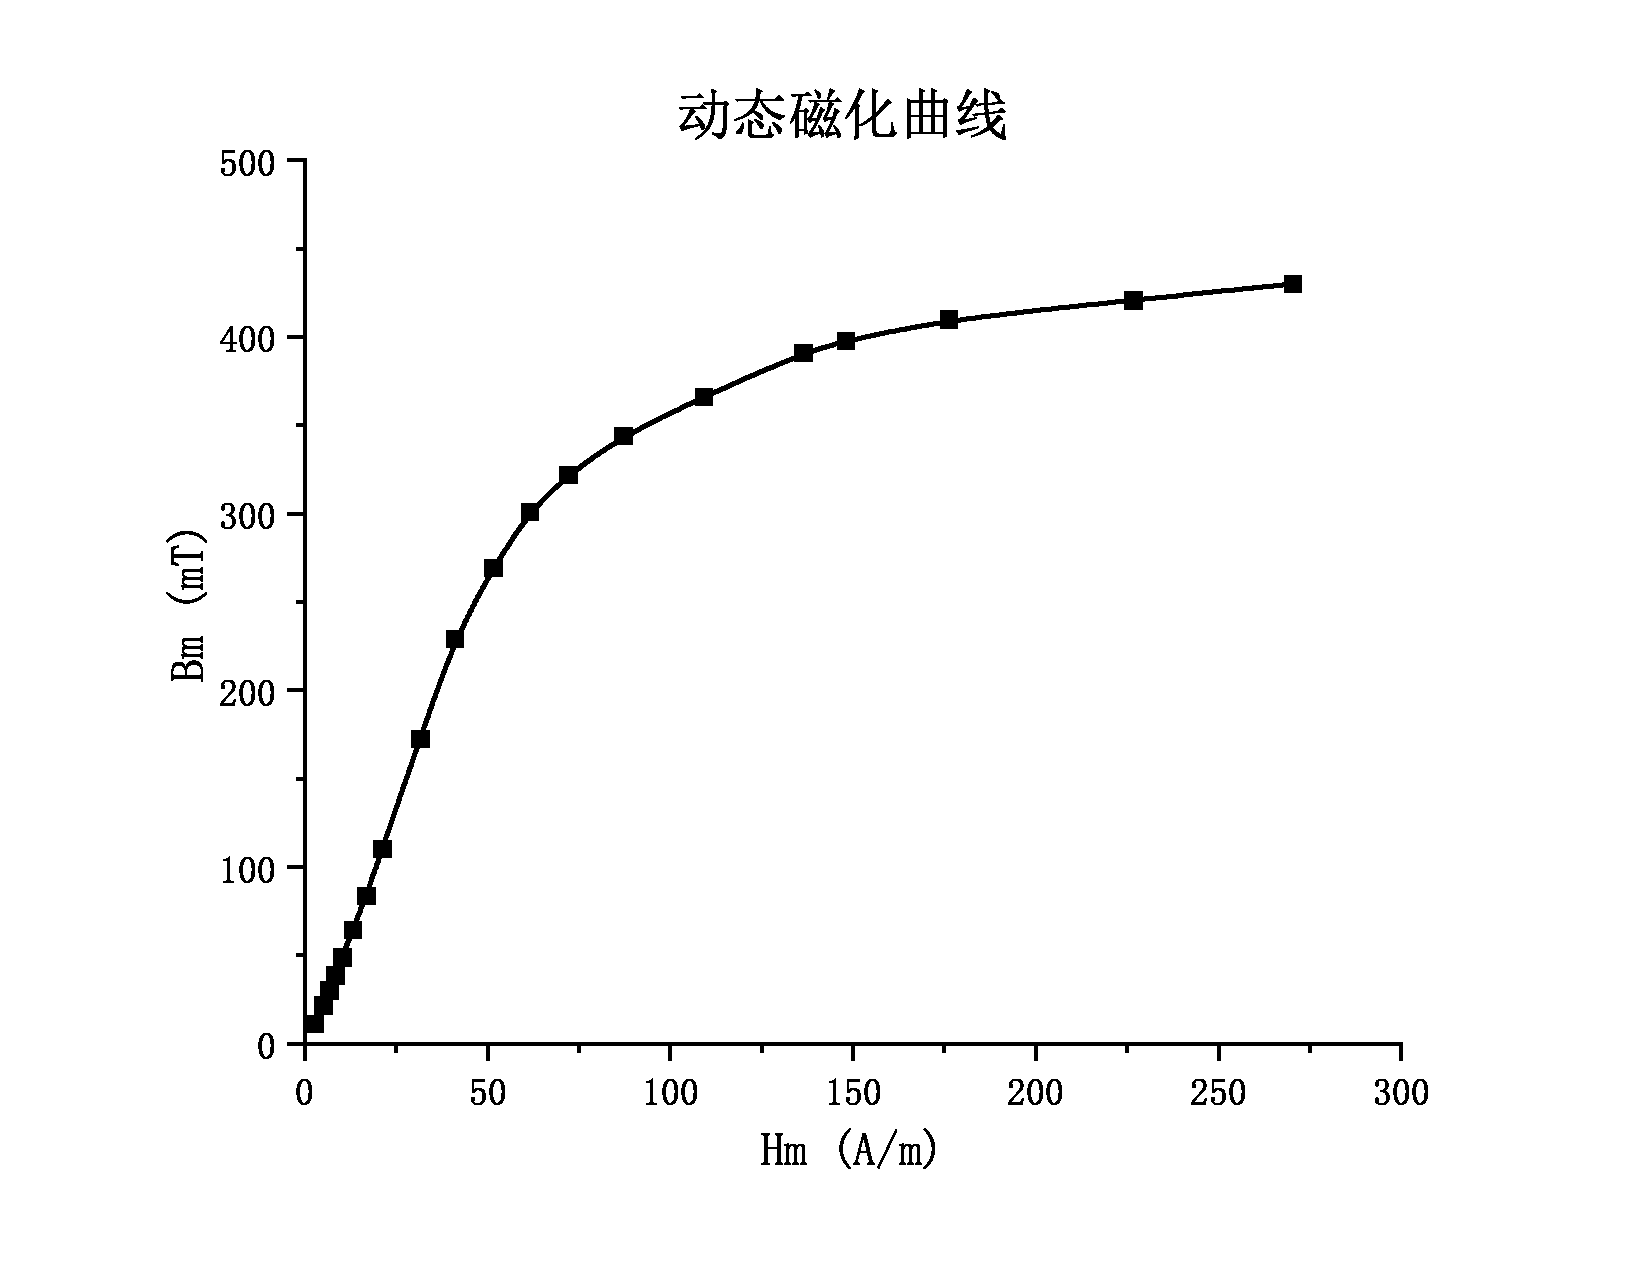
\includegraphics[width=\textwidth]{动态磁化曲线.eps}
            \caption{动态磁化曲线}       
        \end{minipage}
        \begin{minipage}{0.45\textwidth}
            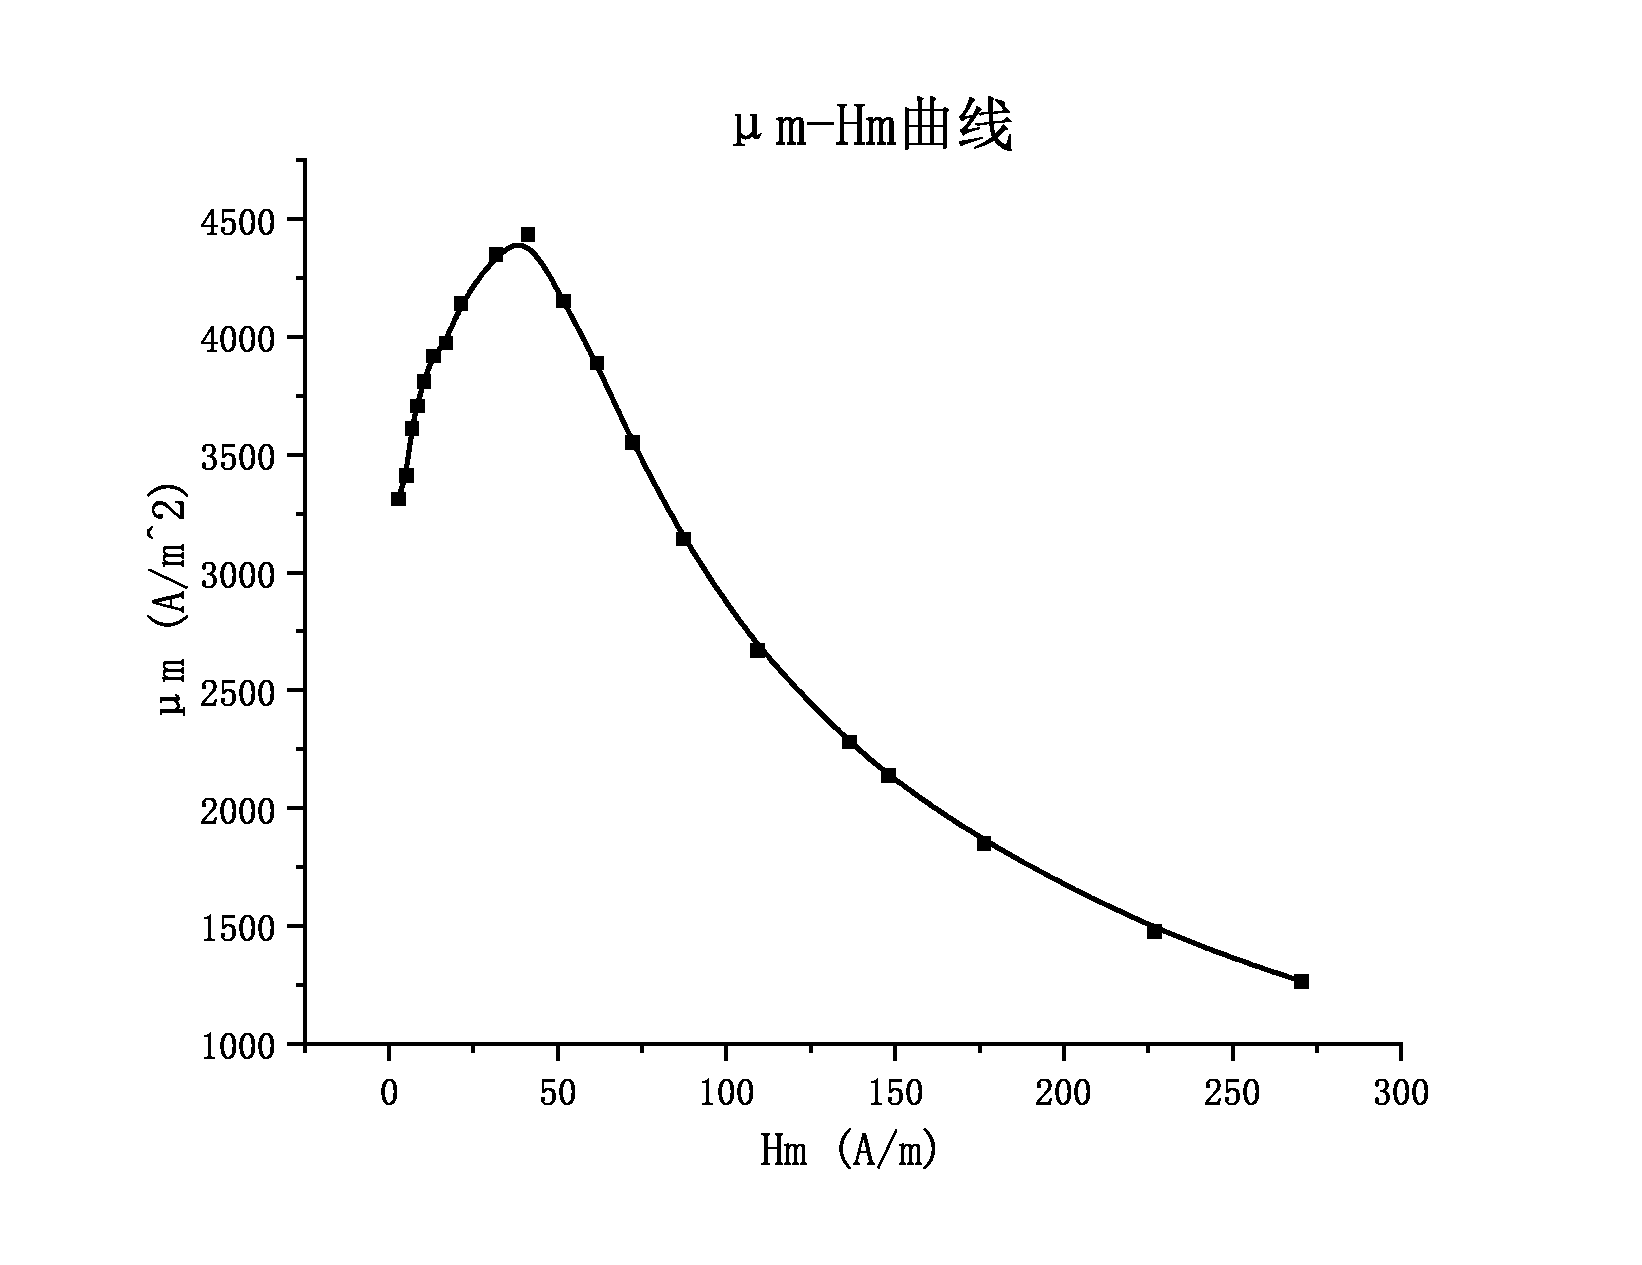
\includegraphics[width=\textwidth]{μm-Hm曲线.eps}
            \caption{$\mu_m-H_m$曲线}
        \end{minipage}
    \end{figure*}

    \subsection{硅钢样品动态磁滞回线}
    保持$H_m=400A/m$,于是相对应的$2u_R=0.8V$,测量硅钢样品在$f=20,40,60Hz$下的$B_m$,$B_r$和$H_c$。

    $f=20Hz:$
    $$2u_m=69.2mV,\ B_m=961mT$$
    $$2u_r=42.8mV,\ B_r=594mT$$
    $$2u_c=208mV,\ H_c=104A/m$$

    $f=40Hz:$
    $$2u_m=69.2mV,\ B_m=961mT$$
    $$2u_r=44.8mV,\ B_r=622mT$$
    $$2u_c=248mV,\ H_c=124A/m$$

    $f=60Hz:$
    $$2u_m=69.0mV,\ B_m=958mT$$
    $$2u_r=46.8mV,\ B_r=650mT$$
    $$2u_c=282mV,\ H_c=141A/m$$

    可以看到,相较于铁氧体的磁滞回线,硅钢的磁滞回线要更大、更“胖”一些。这是因为硅钢电阻率低,涡流损耗较大,磁滞回线所围成的面积较大。
    此外,随着频率的升高,最大点$B_m$几乎不变,剩磁$B_r$和矫顽力$H_c$均有比较明显的增加,这一点与铁氧体也有很大不同。
    这同样是是因为硅钢电阻率低,频率的大小对涡流损耗的影响比铁氧体大,因此剩磁和矫顽力随频率升高而变大的趋势更显著。

    \section{思考题}
    \begin{enumerate}
        \item [(1)] 铁磁材料的动态磁滞回线和静态磁滞回线在概念上有什么区别?铁磁材料的动态磁滞回线的形状和面积受哪些因素影响?\\
        动态磁滞回线是指给铁磁材料加上交变磁场即交变励磁电流时形成的磁滞回线,而静态磁滞回线是加上稳定电流时磁感应强度随磁场强度的变化曲线,
        即动态磁滞回线是励磁电流变化大于一个周期时形成的磁滞回线。铁磁材料的动态磁滞回线的形状主要取决于饱和磁感应强度及其对应磁场强度、矫顽力、剩磁这几个特征量,而这些特征量主要取决于材料。
        而磁滞回线的形状会影响磁滞回线围成的面积,该面积等于磁场变化一周所损耗的能量。能量损耗来自于磁滞损耗、涡流损耗和剩余损耗,这些都与材料的电阻率等特性有关。

        \item [(2)] 铁氧体和硅钢的动态磁化特性各有什么特点?\\
        铁氧体的动态磁滞回线比较“瘦”,硅钢的动态磁滞回线比较“胖”,即硅钢的磁滞回线围成的面积更大;
        此外,铁氧体的磁滞回线随励磁电流频率变化变化不明显,而硅钢的磁滞回线随频率变化会发生较为明显的变化。
        这些特性都与硅钢的电阻率较低,涡流损耗大有关。
        
        \item [(3)] 本实验中,电路参量怎样设置才能保证$u_{R_1}-u_C$所形成的的李萨如图形能正确反应动态磁滞回线的形状?\\
        要保证RC积分电路中的积分常量远大于外电路的变化周期,即$\tau=R_2C\gg T=\frac{1}{f}$,这样才能保证示波器监测的电压与磁感应强度和磁场强度之间是线性关系,即公式
        $$H=\frac{N_{1}}{l R_{1}} u_{R_{1}}\ ,\ B=\frac{R_{2} C}{N_{2} S} u_{C}$$
        成立。

        \item [(4)] 实验中如何判断动态磁滞回线的绕行方向?\\
        磁滞回线的绕行方向是从上半支下降,再从下半支上升。
    \end{enumerate}

\end{document}
